\documentclass[11pt, oneside]{article}   	% use "amsart" instead of "article" for AMSLaTeX format
\usepackage{geometry}                		% See geometry.pdf to learn the layout options. There are lots.
\geometry{letterpaper}                   		% ... or a4paper or a5paper or ... 
%\geometry{landscape}                		% Activate for for rotated page geometry
%\usepackage[parfill]{parskip}    		% Activate to begin paragraphs with an empty line rather than an indent
\usepackage{graphicx}				% Use pdf, png, jpg, or eps§ with pdflatex; use eps in DVI mode
								% TeX will automatically convert eps --> pdf in pdflatex		
\usepackage{amssymb}
\usepackage{indentfirst}

\setlength{\textwidth}{7in}
\setlength{\hoffset}{0pt}
\setlength{\oddsidemargin}{-0.3in}
\setlength{\topmargin}{-1in}
\setlength{\textheight}{9.5in}

\title{Report}
\date{2015/4/10}							% Activate to display a given date or no date

\begin{document}

\maketitle

\section{Implement}
\noindent \textbf{\ \ \ Training}
\begin{enumerate}
\item Make sure the Forward and Backward procedures work properly, which means $P( \bar{O}  | \lambda)$ can be calculated accurately  by either $\alpha_t(i)$ or  $\beta_t(i)$. Then we can iteratively do the following EM steps:
\item \textbf{E-step:} Update $\alpha_t(i), \beta_t(i)$ and calculate $\epsilon_t(i,j), \gamma_t(i)$ using current transition matrix $A, B$ and initial probability $\pi$. 
\item \textbf{M-step:} Re-estimate  $A,B$ and $\pi$ according to the $\epsilon_t(i,j)$ and $\gamma_t(i)$ obtained in E-step.
\item \textbf{Efficiency:} Note that in E-step, the denominators of $\epsilon_t(i,j)$ and $\gamma_t(i)$ are the same, which is $P( \bar{O}  | \lambda)$. So we only need calculate it once. Meanwhile,  in M-step we need accumulate $\epsilon_t(i,j)$ and $\gamma_t(i)$ through all the samples, and for efficient computation, the summation will be completed in E-step.
\end{enumerate}
\textbf{\ \ \ Testing}
\begin{enumerate}
\item \textbf{Viterbi Algorithm:} Keep track $\delta_t(i)$ and dynamically compute the max likelihood.
\end{enumerate}
\section{Execution}
\begin{enumerate}
\item Compile environment: g++ -o2 -std = c++11
\item The execute commands are exactly the same as those in TA's README.  
\item \emph{run.sh} is added to simplify the whole procedure. It can easily get the test accuracy with different training iterations with the help of \emph{compute\_acc.py}.
\item Large iteration numbers (larger than 100) may need a few minutes.
\end{enumerate}
\begin{figure}
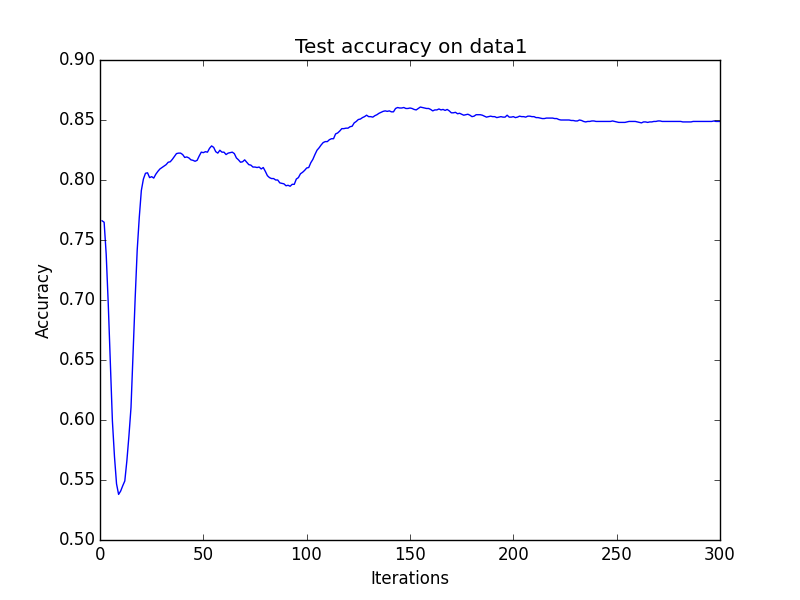
\includegraphics[width=250pt]{exp.png}
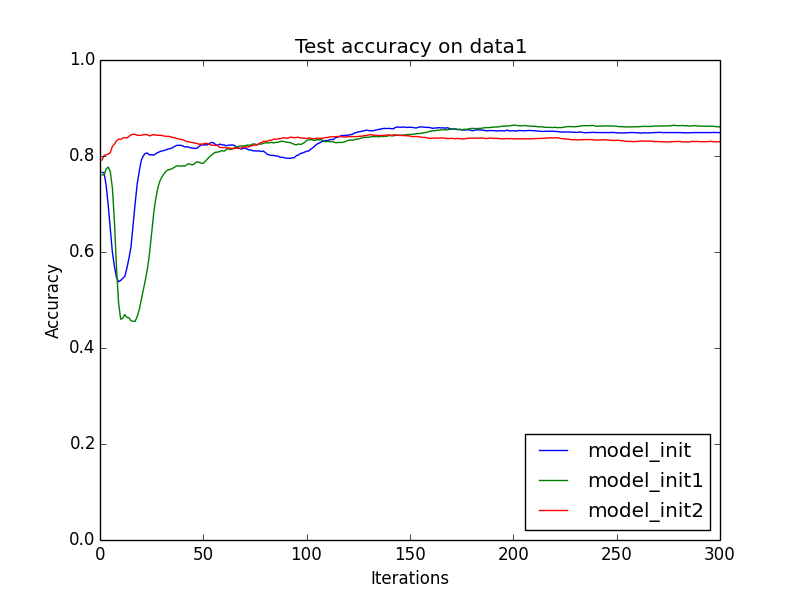
\includegraphics[width=250pt]{exp2.png}
\caption{The left figure (a) shows different testing accuracies with different training iterations, and the right figure (b) shows different accuracies with different initial models.}
\end{figure}
\section{Experiment Results and Analysis}
With the above method, we can estimate the performance of our HMM models by observing the changes of the accuracy when applying different settings, e.g. different number of iterations, different initial models and different number of training samples. According to the experiments, we can infer that Baum-Welch Algorithm will converge with an arbitrary initial model when the iteration number goes large.
\subsection{Number of Iterations}
According to figure 1(a), we can find that with the increase of EM iterations, the test accuracy has a quick decline and rise at the very beginning,  and then goes up gradually with slight oscillation.The best accuracy is 0.8608 at 155 iterations. And when the number of iterations is large enough, the accuracy will reach to a stable value. This tallies with the convergence of EM Algorithm. So we can claim that, as long as we train the HMM model with large enough iterations (around 150 times in our cases), we can always have a relative good result.  Therefore, I used the models trained with 155 iterations to test data2.
\subsection{Initial Model}
Someone may wonder whether the curve of figure 1(a) is typical since the initial model can be changed. So I randomly modified it to another two initial models (seen in the submitted files) to do training. From figure 1(b), we can find that different initial models lead to different accuracies at the beginning, and then they converge to almost the same accuracy after 150 iterations. It infers that Baum-Welch algorithm may have some bias when the iteration number is small, but it can finally converge. Something interesting is that the accuracy of \emph{model\_init1} has a rough decline and rise from 1 to 20 iterations just like the initial model TA provides, while the accuracy of \emph{model\_init2}  increases at first and reaches its best value at the same range of iterations. That means we can get the best accuracy at the very beginning if we could find a better initial model.
\subsection{Number of Samples}
In the class, we discussed Baum-Welch algorithm on one single sequence of observation, but in the experiments, we use many samples to train the model. So what if we do it by one sample at a time? I tried dealing with one sample per iteration,  but found it got low accuracy and has some problems to get the convergence. It might because some of the instances are noisy, they may lead the model farm away from the optimal one, while training with all the samples can avoid this.
\end{document}  